\chapter{Resultados}
\label{chap:resultados}
A fase de desenvolvimento do robô Doogie culminou em 4 resultados principais: Protótipo, ambiente de simulação, labirinto para testes e competição e a estrutura de software da plataforma móvel. Os tópicos posteriores irão detalhar cada um desses resultados. 

%--------- NEW SECTION ----------------------
\section{Protótipo}
\label{sec:resultado_prototipo}

\begin{figure}[H]
	\centering
	\caption{Componentes da placa superior do Doogie Mouse}
	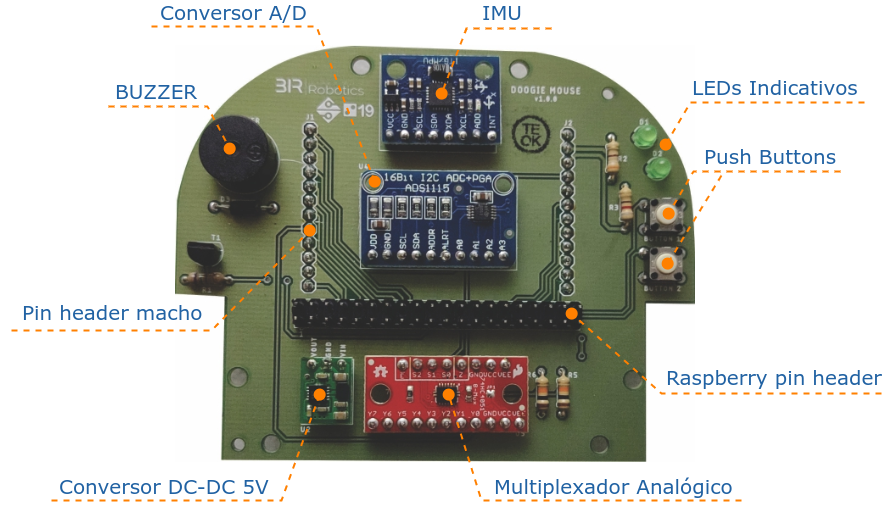
\includegraphics[width=1\textwidth]
	{Figures/top_board_elementos.png}
	\label{fig:top_board_elementos}
	\source{Própria Autoria}
\end{figure}

\begin{figure}[H]
	\centering
	\caption{Componentes da placa inferior do Doogie Mouse}
	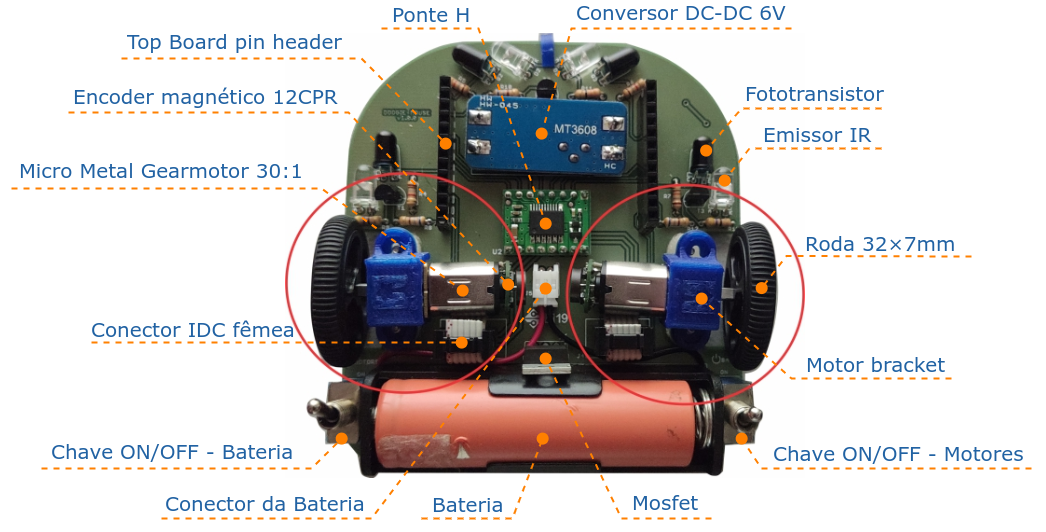
\includegraphics[width=1\textwidth]
	{Figures/bottom_board_elementos.png}
	\label{fig:bottom_board_elementos}
	\source{Própria Autoria}
\end{figure}

\begin{figure}[H]
	\centering
	\caption{Protótipos do Doogie Mouse confeccionados}
	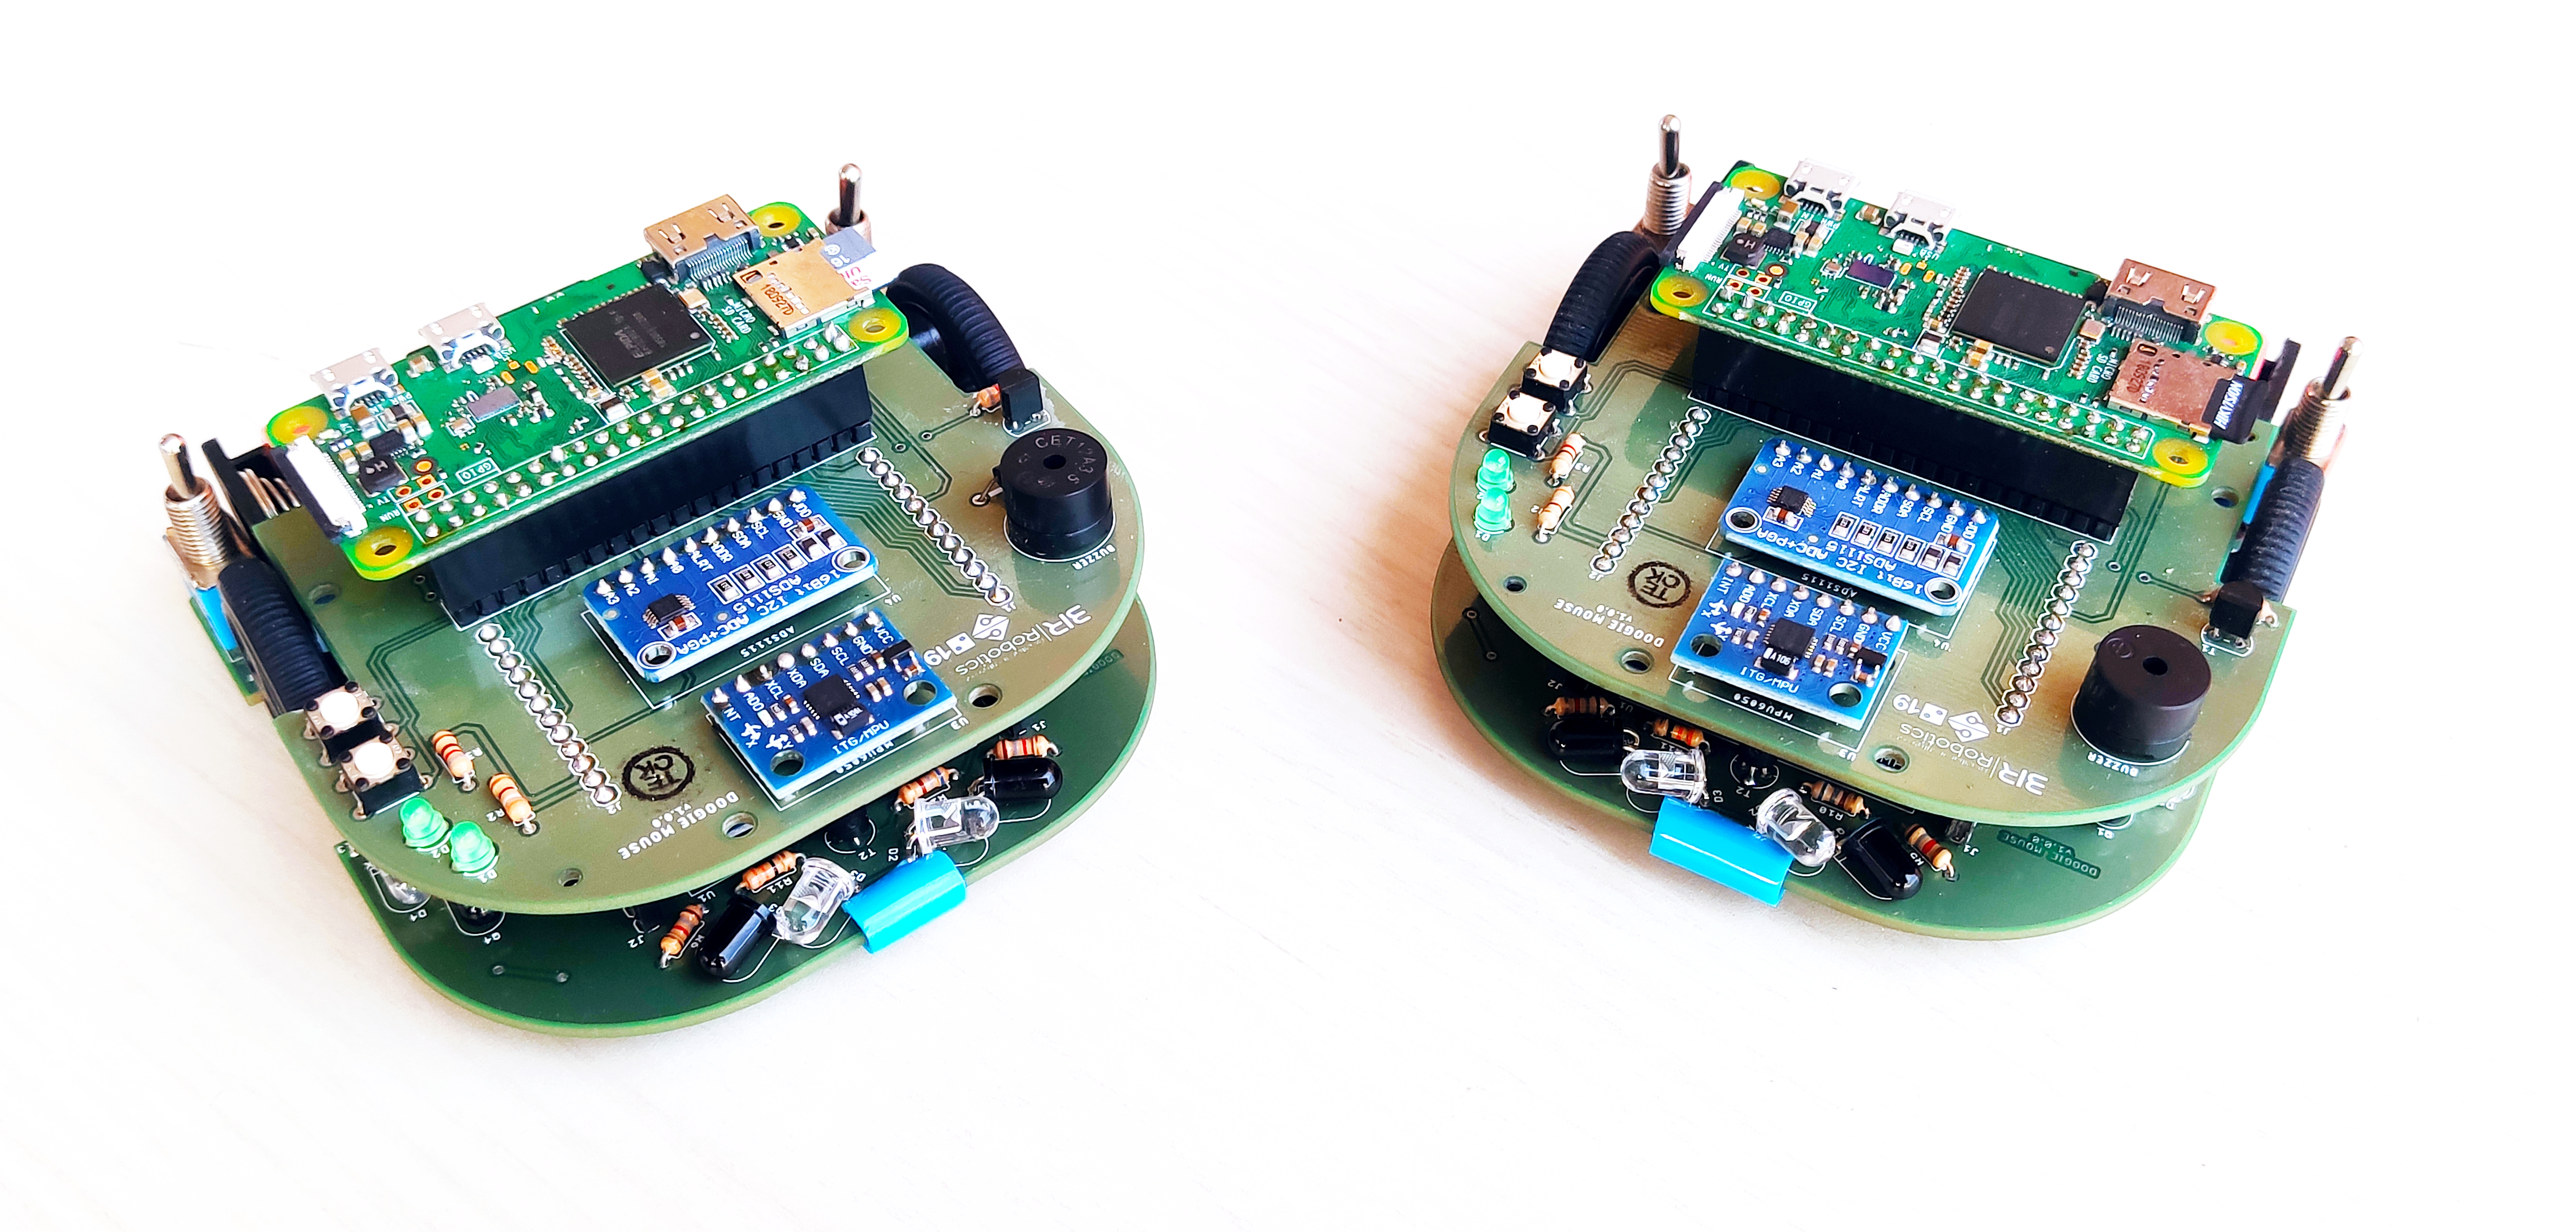
\includegraphics[width=1\textwidth]
	{Figures/doogie_mouse_prototipos}
	\label{fig:prototipos}
	\source{Própria Autoria}
\end{figure}

\section{Ambiente de simulação}
\label{sec:resultado_ambiente_de_simulacao}
hhajshfdsahf

%--------- NEW SECTION ----------------------
\section{Labirinto}
\label{sec:resultado_labirinto}
asdfadsfsdfs

%--------- NEW SECTION ----------------------
\section{Estrutura de Software}
\label{sec:resultado_estrutura_de_software}
Para contemplar o objetivo do projeto, que é ser uma plataforma para aprendizagem de robótica móvel e inteligência artificial, optou-se pelo uso do \textit{framework} \gls*{ros} devido a sua capacidade de abstração de hardware e de reuso de software como já mencionado em \ref{sec:robotic_frameworks}. Diante disso, foi criada uma estrutura de software modular que pode ser visualizada na Figura \ref{fig:doogie_packages}. Essa estrutura é formada por \textit{stacks}, que são conjunto de pacotes agrupados em um mesmo local. Abaixo está descrito qual o objetivo de cada pacote dentro dessas \textit{stacks}.

\textbf{doogie\_base}:
\begin{itemize}
	\item \textbf{doogie\_algorithms}: Contém os algoritmos de inteligência que são utilizados pelo robô na resolução do labirinto;
	\item \textbf{doogie\_control}: Possui arquivos de configuração e de inicialização dos processos de controle do robô;
	\item \textbf{doogie\_description}: Abarca arquivos com a descrição do modelo do robô;
	\item \textbf{doogie\_msgs}: Compreende as estrutura de dados (.msg e .action) criadas exclusivamente para o Doogie Mouse;
	\item \textbf{doogie\_navigation}: Abrange os processos utilizados para a percepção, localização e navegação do robô dentro do labirinto. Fornece também \glspl*{api} para permitir que usuários implementem sua própria estratégia de resolução de labirinto.   
\end{itemize}
	
\textbf{doogie\_simulator}:
\begin{itemize}
	\item \textbf{doogie\_gazebo}: Integra todos os arquivos de configuração necessários para executar o ambiente de simulação.
\end{itemize}
	
\textbf{doogie\_robot}
\begin{itemize}
	\item \textbf{doogie\_bringup}: Agrupa arquivos de configuração e inicialização de todos os subsistemas do robô. Contém também os executáveis responsáveis pela atuação da plataforma móvel.  
	\item \textbf{doogie\_drivers}: Compreende executáveis e bibliotecas dos componentes de hardware do robô (motor, Encoder, \gls*{imu} e sensores infravermelho).
\end{itemize}
	
\textbf{doogie\_desktop}
\begin{itemize}
	\item \textbf{doogie\_rviz}: Engloba arquivos de configuração e inicialização para visualização de dados do robô no visualizador RViz;
	\item \textbf{doogie\_welcome}: Contém executáveis para verificação do funcionamento do \textit{framework} ROS na etapa de instalação.
\end{itemize}

\begin{figure}[H]
	\centering
	\caption{Organização dos pacotes do Doogie Mouse.}
	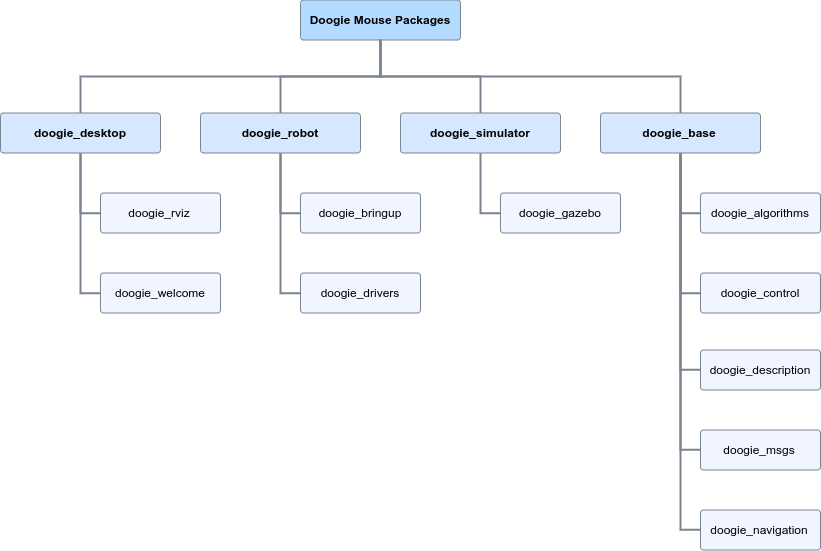
\includegraphics[width=1\textwidth]
	{Figures/doogie_packages}
	\label{fig:doogie_packages}
	\source{Própria Autoria}
\end{figure}

Dentre as \textit{stacks} e pacotes listados na Figura \ref{fig:doogie_packages} apenas a \textit{stack} doogie\_desktop e o pacote doogie\_rviz não foram criados. Os demais estão disponíveis para utilização no repositório remoto GitHub.

Embora todos esses pacotes tenham sido criados, nem todos eles são empregados no funcionamento da plataforma móvel. Como alguns pacotes são utilizados apenas para simulação do robô, não há a necessidade da sua utilização dentro da plataforma. Dessa forma, os pacotes foram organizados de acordo com o propósito final: utilização no ambiente de simulação, no robô físico ou em ambos. A Figura \ref{fig:diagrama_dos_pacotes} demonstra como esses pacotes se relacionam entre si. A \textit{stack} doogie\_base é comum tanto ao ambiente de simulação quanto ao robô físico, porém, não tem utilidade se não utilizada dentro desses dois contextos. A \textit{stack} doogie\_robot possui todos os pacotes essenciais para o funcionamento do robô físico, entretanto, possui dependência direta com a \textit{stack} doogie\_base. Em oposição está a \textit{stack} doogie\_simulator válida apenas para uso do ambiente de simulação, mas igualmente a doogie\_robot, depende da doogie\_base para funcionar. Englobando todas as \textit{stacks} mencionadas bem como a reunião de toda a documentação do robô está a \textit{stack} doogie\_desktop. A relação de dependência entre esses pacotes é feita através de arquivos de configuração que são utilizados no processo de compilação dos pacotes através de ferramentas específicas do \textit{framework} ROS. Caso uma dependência não seja satisfeita, por exemplo uma \textit{stack} não instalada, um erro ocorrerá.   

\begin{figure}[H]
	\centering
	\caption{Relação de dependência das \textit{stacks} do Doogie Mouse.}
	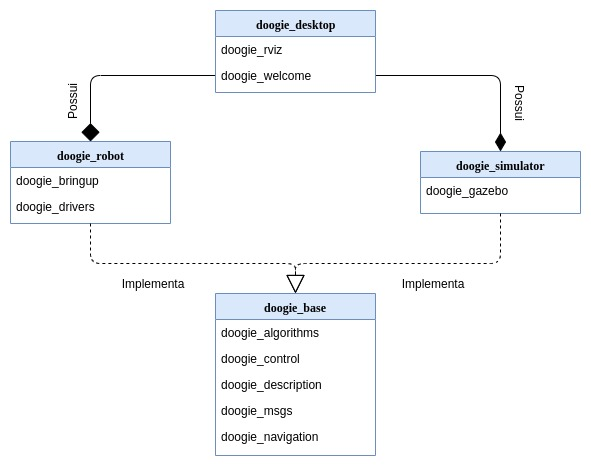
\includegraphics[width=1\textwidth]
	{Figures/diagrama_dos_pacotes}
	\label{fig:diagrama_dos_pacotes}
	\source{Própria Autoria}
\end{figure}

Continuando com a proposta de modularidade de sistemas para proporcionar um grau de flexibilidade no uso de diferentes estratégias de resolução do labirinto, foi pensado, embora não testado, um modelo de comunicação entre os processos dentro do ambiente \gls*{ros}, conforme ilustrado pela Figura \ref{fig:doogie_ros_graph}.

\begin{figure}[H]
	\centering
	\caption{Diagrama de comunicação entre processos.}
	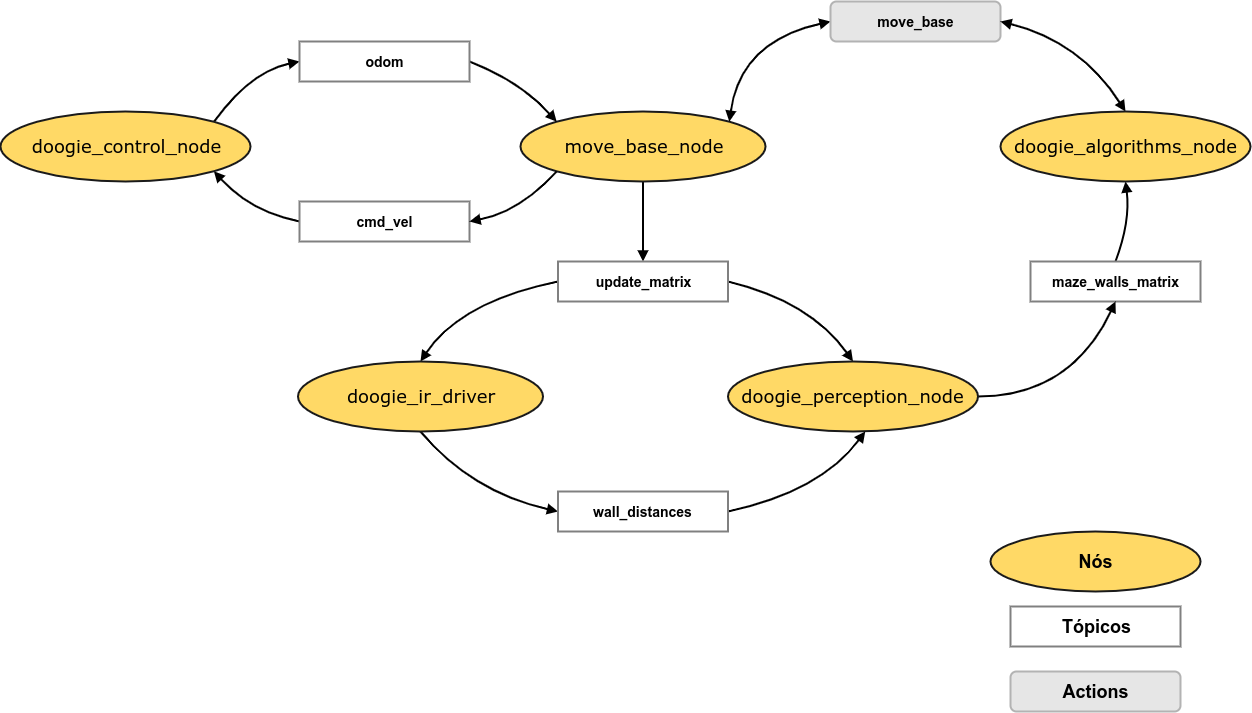
\includegraphics[width=1\textwidth]
	{Figures/doogie_ros_graph}
	\label{fig:doogie_ros_graph}
	\source{Própria Autoria}
\end{figure}

Partindo da premissa que a posição e orientação inicial da base móvel dentro do labirinto é conhecida, a movimentação do robô começa com o doogie\_algorithms\_node enviando um comando de movimentação para o move\_base\_node. Após interpretado qual movimento a plataforma deve executar, o processo move\_base\_node enviará valores de velocidade linear e angular através do tópico cmd\_vel para o processo responsável pelo controle de movimentação do robô. Com o \textit{feedback} de Odometria, o move\_base\_node infere se o robô chegou ao destino desejado. Enquanto o robô está se movimentando, uma informação de progresso é enviada para o doogie\_algorithms\_node de modo que ações possam ser tomadas enquanto o robô se locomove, como emitir uma alerta sonoro quando 90\% do trajeto for concluído																																																																																																																																																																																																																																																																																					.Quando o robô chega ao seu destino final (uma determinada célula do labirinto), uma informação de posição e orientação do robô é fornecida através do tópico update\_matrix. Essa informação é armazenada pelo processo de percepção e dispara também uma requisição para que os dados dos sensores infravermelhos sejam fornecidos. Após a requisição de dados, o \textit{driver} dos sensores infravermelho irá providenciar no tópico wall\_distances as informações de distância das paredes do labirinto. Com os valores de distância, posição e orientação do robô, o processo doogie\_perception\_node sintetiza uma matriz de obstáculos fornecendo em relação a um referencial global quais paredes existem para cada célula do labirinto visitada. Essa matriz é então fornecida para o processo que contém a estratégia de resolução do labirinto escolher a próxima ação de movimentação do robô. Essas etapas se repetem até que o robô encontre o centro do labirinto.

Com essa proposta de organização de comunicação entre processos e de posse das \glspl*{api} fornecidas para envio de comandos de movimentação do robô e manuseio da matriz de obstáculos, o usuário pode implementar sua própria estratégia de resolução de labirinto. O fator limitante de qual abordagem dentro da IA utilizar será apenas o poder de processamento da Raspberry Pi.